\chapter{Sztuczna inteligencja}

% http://www.if.pw.edu.pl/~julas/TEXT/pliki/TEXT4.pdf
Koncepcja nowoczesnej sztucznej inteligencji ma swoje korzenie już w pracach klasycznych filozofów, którzy próbowali opisać proces ludzkiego myślenia jako mechaniczną manipulację symbolami.
Wiele wieków później, w latach 40. XX wieku, zwieńczeniem tych prac było wynalezienie programowalnego komputera cyfrowego bazującego na abstrakcyjnym rozumowaniu matematycznym. Urządzenie to i stojące za nim pomysły zainspirowały naukowców do dyskusji na temat możliwości zbudowania „mózgu elektronicznego”.
Badania w tej dziedzinie znacznie przyspieszyły i zróżnicowały się (rozgałęziły) począwszy od lat 50-tych XX wieku, kiedy to Alan Turing --- znany angielski matematyk, kryptolog --- stworzył maszynę Turinga  ---  abstrakcyjny model urządzenia służącego do wykonywania różnych algorytmów. Turing jest uważany za jednego z „ojców” informatyki i sztucznej inteligencji \cite{turing}. W ramach badań nad sztuczną inteligencją zaproponował on wykonanie testu zwanego Testem Turinga, który miał za zadanie sprawdzić czy „wypowiedzi” odpowiednio zaprogramowanej maszyny/algorytmu naśladującego sposób myślenia ludzkiego i posługującego się językiem naturalnym są odróżnialne od wypowiedzi prawdziwego człowieka. Test uznawany jest jako zaliczony, gdy sędzia (człowiek) konwersujący z kilkoma innymi obiektami (kilkoma ludźmi i maszyną) nie jest w stanie stwierdzić, czy w danej chwili rozmawia z człowiekiem, czy z maszyną symulującą człowieka. Od tego ważnego wydarzenia dynamika badań nad przetwarzaniem języka naturalnego (NLP) znacznie przyspieszyła. Ważniejsze kamienie milowe przedstawione są na osi czasu na następnej stronie. Obejmuje ona historię NLP od roku 1950 do czasów obecnych. \\
\noindent W ogólności sztuczna inteligencja jest definiowana jako zdolność systemu do poprawnej interpretacji danych zewnętrznych, uczenia się na podstawie takich danych oraz wykorzystywania tych informacji do osiągania konkretnych celów i zadań wykorzystując elastyczną adaptację \cite{KAPLAN2019}. Sztuczną inteligencję, ze względu na możliwości rozwiązywania przez nią problemów oraz umiejętność dostosowywania się do różnego rodzaju zadań, można podzielić na 3 rodzaje: słabą, ogólną i superinteligencję. \\


%%    http://www.cs.put.poznan.pl/amichalski/wsi/AI1.rgb.pdf


% --------------- TIMELINE ----------------
\startchronology
[
align=left, 
startyear=1950,
stopyear=2021, 
startdate=true, 
stopdate=true, 
dateselevation=-20pt, 
arrow=false,
arrowcolor=black, 
box=true
]

% lata 50-te
\chronoevent[markdepth=-30pt, textwidth=2.5cm, date=false]{1950}{{\small \begin{center}
			\textbf{1950} \\ Test Turinga \cite{turingtesttimeline}
\end{center}}}

% 60-te
\chronoperiode[color=babyblueeyes, startdate=false, stopdate=false]{1956}{1962}{}

\chronoevent[markdepth=20pt, textwidth=3.5cm, date=false]{1959}{{\small \begin{center}
			\textbf{późnie lata 50-te i~wczesne 60-te} \\ sieci semantyczne do tłumaczeń maszynowych \\ \cite{siecisemantyczne}
\end{center}}}
\chronoevent[markdepth=-30pt, textwidth=2.5cm, date=false]{1965}{{\small \begin{center}
			\textbf{1965} \\ ELIZA \\ \cite{eliza}
\end{center}}}

% lata 70-te
\chronoevent[markdepth=20pt, textwidth=2.5cm, date=false]{1975}{{\small \begin{center}
			\textbf{1975} \\ PARRY \\ model paranoika (Colby)
\end{center}}}



% 80-te


\chronoevent[markdepth=-30pt, textwidth=2.5cm, date=false]{1986}{{\small \begin{center}
			\textbf{1986} \\ STUDENT \\ znacznie pojedyńczych słów (Bobrow)
\end{center}}}




\chronoevent[markdepth=20pt, textwidth=2.5cm, date=false]{2011}{{\small \begin{center}
			\textbf{2011}  \\ Watson (IBM) wygrywa w Jeopardy! \\ \cite{jeopardy}
\end{center}}}

\chronoperiode[color=babyblueeyes, startdate=false, stopdate=false]{2011}{2015}{}

\chronoevent[markdepth=-30pt, textwidth=2.5cm, date=false]{2013}{{\small \begin{center}
			\textbf{2011-2014} \\ Apple Siri, asystent Google'a, MS Cortana
\end{center}}}



\stopchronology






%% --------------- TIMELINE ----------------
%\startchronology
%[
%align=left, 
%startyear=1950,
%stopyear=2030, 
%startdate=false, 
%stopdate=false, 
%dateselevation=0pt, 
%arrow=true,
%arrowcolor=babyblueeyes, 
%box=true
%]
%%\chronoperiode[color=darkerBlue, startdate=false, stopdate=false]{1950}{2030}{}
%
%
%% lata 50-te
%\chronoevent[markdepth=-80pt, textwidth=2.5cm, date=false]{1956}{{\small \begin{center}
%			\textbf{1956} \\ Pojęcie sztucznej inteligencji \cite{KAPLAN2019}
%\end{center}}}
%\chronoevent[markdepth=10pt, textwidth=2.5cm, date=false]{1950}{{\small \begin{center}
%			\textbf{1950} \\ Test Turinga \cite{turingtesttimeline}
%\end{center}}}
%
%% 60-te
%\chronoevent[markdepth=60pt, textwidth=3.5cm, date=false]{1958}{{\small \begin{center}
%			\textbf{późnie lata 50-te i~wczesne 60-te} \\ sieci semantyczne do tłumaczeń maszynowych \\ \cite{siecisemantyczne}
%\end{center}}}
%\chronoevent[markdepth=-30pt, textwidth=2.5cm, date=false]{1965}{{\small \begin{center}
%			\textbf{1965} \\ ELIZA \\ \cite{eliza}
%\end{center}}}
%
%% lata 70-te
%\chronoevent[markdepth=10pt, textwidth=2.5cm, date=false]{1974}{{\small \begin{center}
%			\textbf{1974-1980} \\ I. zima AI
%\end{center}}}
%
%\chronoevent[markdepth=-125pt, textwidth=2.5cm, date=false]{1970}{{\small \begin{center}
%			\textbf{1970} \\ propagacja wsteczna
%\end{center}}}
%
%
%% 80-te
%\chronoevent[markdepth=60pt, textwidth=2.5cm, date=false]{1984}{{\small \begin{center}
%			\textbf{1984} \\ Film Terminator
%\end{center}}}
%
%\chronoevent[markdepth=-70pt, textwidth=2.8cm, date=false]{1980}{{\small \begin{center}
%			\textbf{1980-1987} \\ Rozwój AI w~Wlk. Brytanii
%\end{center}}}
%
%\chronoevent[markdepth=-30pt, textwidth=2.5cm, date=false]{1990}{{\small \begin{center}
%			\textbf{1987-1993} \\ II. zima AI
%\end{center}}}
%
%
%
%% lata 90-te
%\chronoevent[markdepth=10pt, textwidth=2.5cm, date=false]{1997}{{\small \begin{center}
%			\textbf{1997} \\ Deep Blue (IBM) pokonuje Garego Kasparova w~szachy
%\end{center}}}
%
%
%
%% 2000-czne
%\chronoevent[markdepth=-100pt, textwidth=2.5cm, date=false]{2001}{{\small \begin{center}
%			\textbf{2001} \\ Film A.I. Steven'a Spielberg'a
%\end{center}}}
%
%
%\chronoevent[markdepth=-30pt, textwidth=1.5cm, date=false]{2009}{{\small \begin{center}
%			\textbf{2010} \\ Kinnect XBOX (CV)
%\end{center}}}
%
%
%
%
%
%\chronoevent[markdepth=90pt, textwidth=2.5cm, date=false]{2019}{{\small \begin{center}
%			\textbf{2015} \\ AlphaGo pokonuje mistrza w Go
%\end{center}}}
%
%
%\chronoevent[markdepth=10pt, textwidth=2.3cm, date=false]{2011}{{\small \begin{center}
%			\textbf{2011}  \\ Watson (IBM) wygrywa w Jeopardy
%\end{center}}}
%
%\chronoevent[markdepth=-100pt, textwidth=2.5cm, date=false]{2014}{{\small \begin{center}
%			\textbf{2011-2014} \\ Apple Siri, asystent Google'a, MS Cortana
%\end{center}}}
%
%\chronoevent[markdepth=-30pt, textwidth=2.2cm, date=false]{2021}{{\small \begin{center}
%			\textbf{2017} \\ konferencja o etyce w AI
%\end{center}}}
%
%
%\chronoevent[markdepth=10pt, textwidth=2cm, date=false]{2026}{{\small \begin{center}
%			\textbf{2020}  \\  GPT-3 (OpenAI)
%\end{center}}}
%
%
%\stopchronology




%
%
%\textcolor{TODO}{Potem napisać jak przez lata rozwijała się sztuczna inteligencja - jakiś krótki rys historyczny i kiedy tak naprawdę zaczął się dynamiczny rozwój - coraz mocniejsze komputery, coraz tańsze przetwarzanie, zasoby do przechowywania itd. Jak obecnie dzieli się sztuczną inteligencję (general, super, itd. - 3 rodzaje). Jakie są wady i jakie potencjalne zagrożenia mogą być z nią związane. Jakie są zalety AI i technologii powiązanych. Co można wyciągnąć i w jaki sposób wykorzystuje się dane - jakie sektory, po co, jakie korzyści biznesowe i niebiznesowe za tym idą itd. Analiza, wizualizacja - jak i po co? Rodzaje technologii - ML, NN, CV, NLP itd. i do czego są wykorzystywane. TO CO PONIŻEJ WRZUCIĆ JAK JUŻ BĘDĘ PRÓBOWAŁA NAWIĄZAĆ DO NLP. Dobór techniki opiera się na tym, z jakimi danymi mamy do czynienia. Napisać też o danych generowanych z różnych urządzeń pomiarowych i czujników, smart homes, zegarki, rózne pulsomierze i inne pierdoły (wspomnieć).} \\




\bigskip

%   http://www.cs.put.poznan.pl/amichalski/wsi/AI1.rgb.pdf
\noindent Głównymi obszarami zastosowań sztucznej inteligencji są:
\begin{itemize}
\item uczenie maszynowe (automatyczne),
\item rozpoznawanie i przetwarzanie obrazów --- diagnostyka medyczna, tworzenie gier, śledzenie, tworzenie sztuki,
\item \textbf{przetwarzanie języka naturalnego (NLP)},
\item robotyka i planowanie działań,
\item tworzenie systemów eksperckich.
\end{itemize}

%%%  ------------> obrazek
%\begin{figure}[H]
%	\centering
%	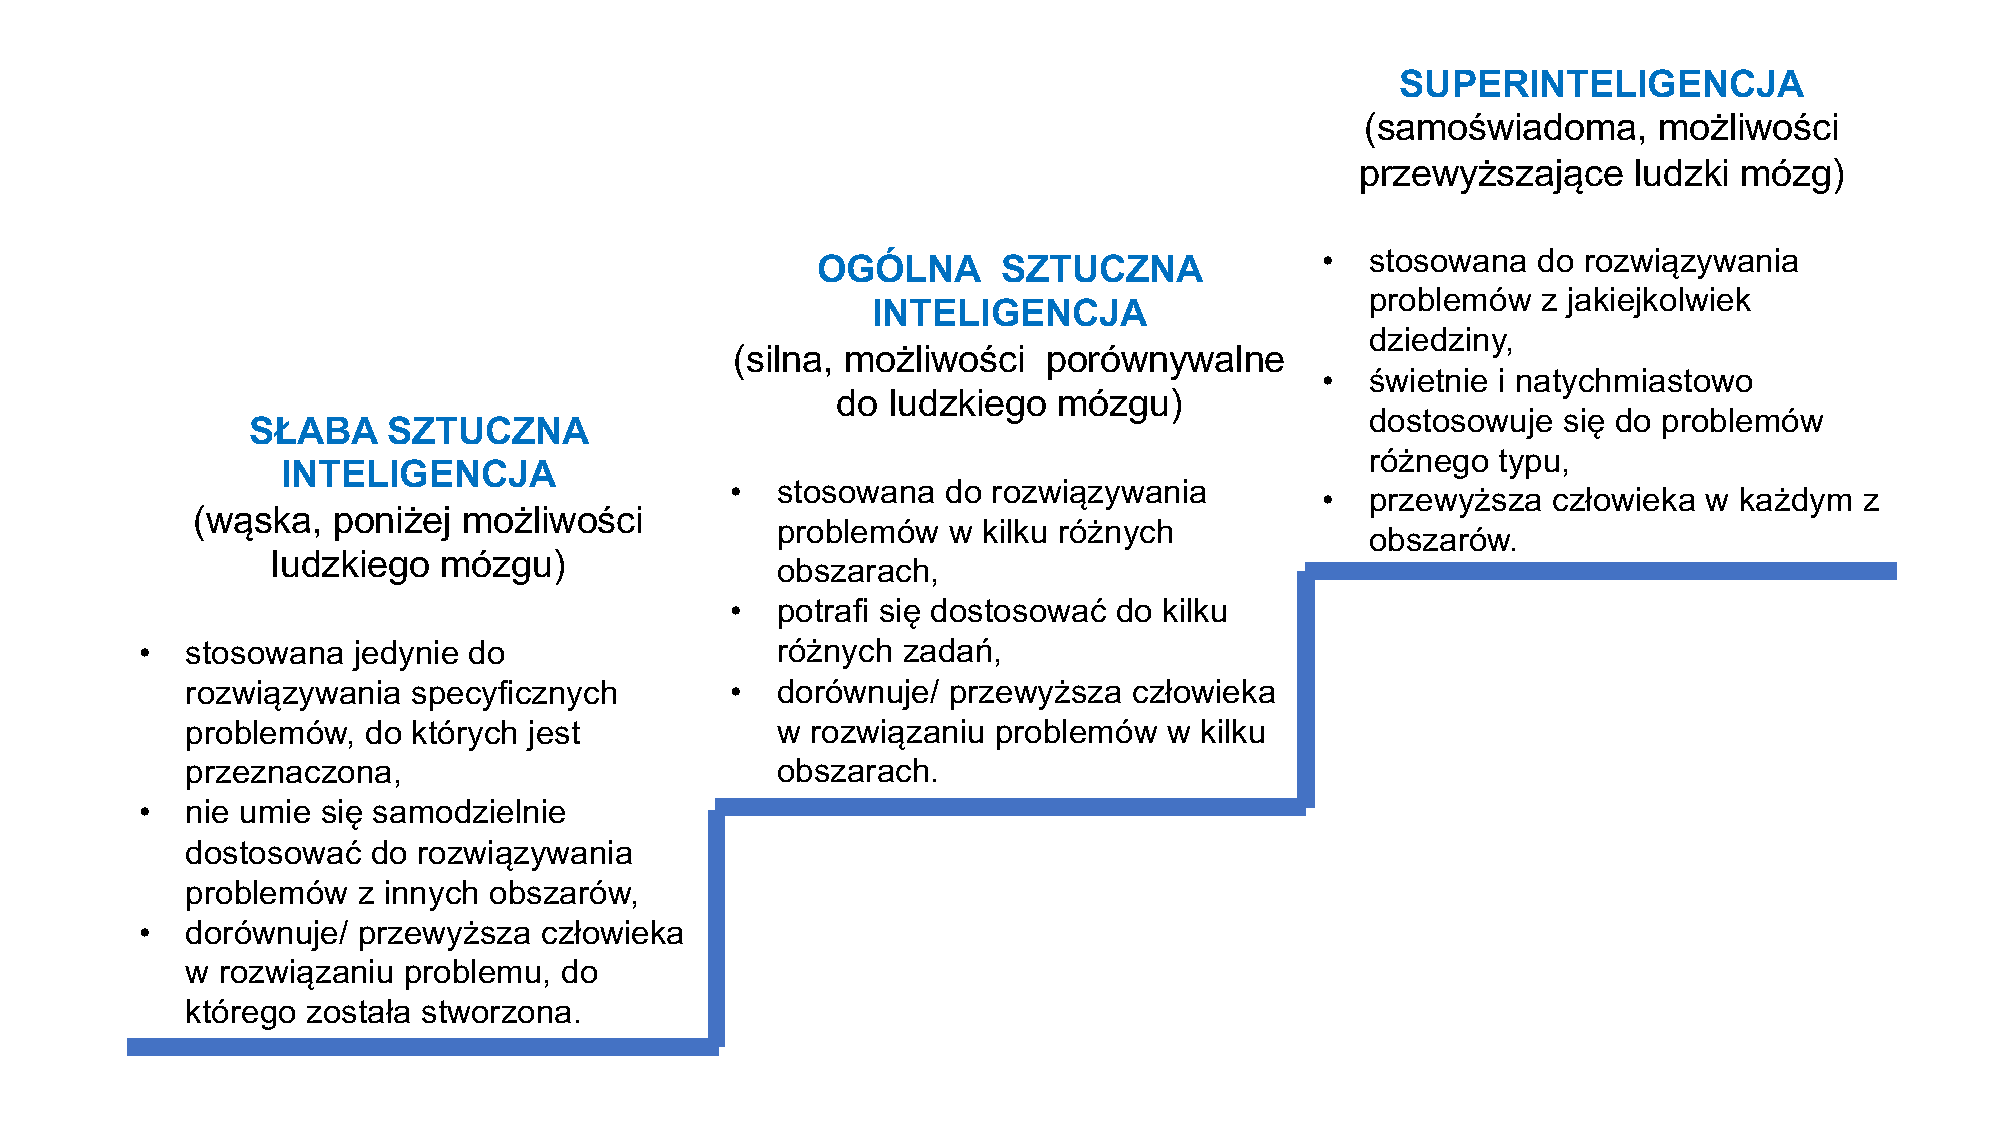
\includegraphics[width=0.95\linewidth]{images/chapter1/weak-general-super-intelligence.pdf}
%	\caption{Rodzaje i możliwości współczesnej sztucznej inteligencji.}
%	\label{fig:narrow-general-super}
%\end{figure}

\bigskip

\noindent Obecnie świat napędzany jest nieustannie rosnącą ilością generowanych danych.  W 2020 roku zostało wygenerowanych, prztworzonych, skopiowanych lub pobranych ponad 64 zettabajy danych. Jeden zettabajt danych, to 10$^{21}$ bajtów. Odnosząc się do danych podawanych przez platformę \copyright~Statista, prognozowana ilość danych ma się mniej więcej potroić do końca 2025 roku \cite{Statista}. Ze względu na tą ogromną ilość ważne jest aby stworzyć efektywne systemy umożliwiające jej wykorzstywanie.


%%%  ------------> obrazek z podpisem hyperlinkiem
%\begin{figure}[H]
%	\centering
%	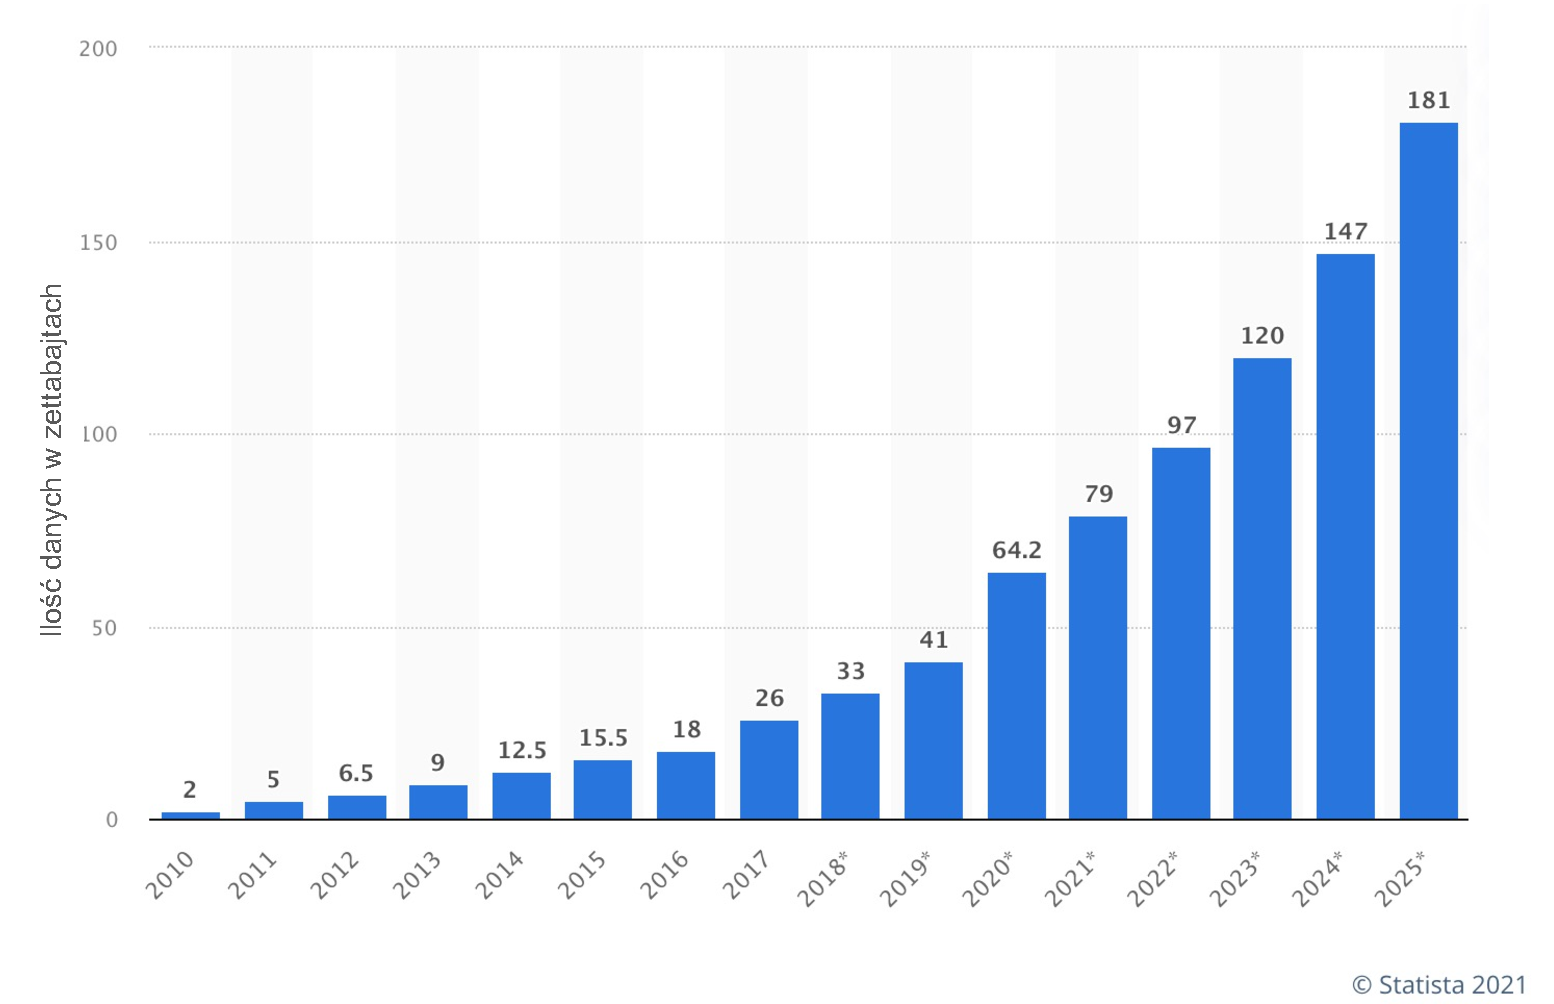
\includegraphics[width=0.95\linewidth]{images/chapter1/data-volume.pdf}
%	\caption{\href{https://www.statista.com/statistics/871513/worldwide-data-created/}{Ilość danych przetwarzanych rocznie w latach 2010 -- 2025.}}
%	\label{fig:data-volume}
%\end{figure}


% z prezentacji

\noindent Wg różnych źródeł \cite{unstructuredData}, około 80\% danych generowanych w obecnych czasach występuje w formie nieustrukturyzowanej, np. jako posty na Facebooku, tweety, opinie, recenzje wystawiane przez użytkowników na portalach internetowych, nagrania audio, wiadomości z Messengera czy Whatsappa oraz dane zbierane przez asystentów głosowych typu Alexa, Siri Cortana itd.
Do danych nieustrukturyzowanych zaliczamy też filmy oraz zdjęcia i wszelką grafikę.
Jednak ze względu na potrzeby tej pracy, skupimy się na danych tekstowych. \\

\noindent Dane nieustrukturyzowane niosą ze sobą mnóstwo użytecznych informacji. Jednak ze względu na nieodłączną złożoność ich przetwarzania i analizowania, praca z nimi stanowi wyzwanie, gdyż dane te trzeba najpierw skrupulatnie wydobyć z surowych zbiorów (nieobrobionych danych źródłowych) lub różnego rodzaju rejestratorów. Jednakże uważamy, że warto poświęcić na to czas, gdyż z biznesowego punktu widzenia nieustrukturyzowane dane stanowią potencjalną kopalnią złota.

\noindent Dla porównania, dane ustrukturyzowane czyli takie, które posiadają konkretną ściśle zdefiniowaną formę stanowią jedynie około 20\% wszystkich generowanych danych, a więc zdecydowaną mniejszość. Jest to kolejny powód, dla którego warto sięgać też po dane nieustrukturyzowane, gdyż korzystanie tylko z tych ustrukturyzowanych danych powoduje, że dużo wartości umyka.
Oba rodzaje wspomnianych danych wykazują istotne różnice. Poniżej wymienione są te najważniejsze.

\begin{table} [H]
	\caption{Porównanie danych ustrukturyzowanych i nieustrukturyzowanych.}
\begin{center}
	\begin{tabular}{ |p{7cm}|p{7cm}|  }
		\hline
		\begin{center}
			Dane ustrukturyzowane 
		\end{center}& \begin{center}
		Dane nieustrukturyzowane
	\end{center} \\  
		\hline
		\ding{70} o jasno zdefiniowanych typach, które można przeszukiwać wg określonych kryteriów & \ding{70} zwykle przechowywane w ich natywnym formacie \\ 
		\ding{70} najczęściej ilościowe & \ding{70} najczęściej jakościowe \\ 
		\ding{70} często przechowywane w hurtowniach danych & \ding{70} często przechowywane w jeziorach danych \\ 
		\ding{70} można je łatwo przeszukiwać i analizować & \ding{70} wymagają więcej pracy --- wstępnej obróbki --- do wydobycia i zrozumienia informacji, które niosą \\ 
		 \ding{70} istnieją we wstępnie zdefiniowanych formatach & \ding{70} występują w różnych formatach \\  
		\hline
	\end{tabular}
\end{center}
\end{table}

\noindent Ze względu na cel niniejszej pracy, skupimy się na możliwościach przetwarzania i analizowania danych w postaci tekstu pisanego (recenzji filmów). Będziemy opierać się na koncepcji przetwarzania języka naturalnego.


\section{Przetwarzanie języka naturalnego}

Dane nie posiadające zdefiniowanej struktury --– w szczególności te tekstowe i głosowe można analizować przy pomocy przetwarzania języka naturalnego.
Wg Wikipedii: przetwarzanie języka naturalnego (\textit{Natural Language Processing}, NLP) to interdyscyplinarna dziedzina, łącząca zagadnienia sztucznej inteligencji i językoznawstwa, zajmująca się automatyzacją języka naturalnego przez komputer, w tym analizą, rozumieniem, tłumaczeniem i generowaniem języka naturalnego \cite{wikipediaNLP}. 
%Systemy rozumiejące język naturalny przekształcają próbki języka naturalnego na bardziej formalne symbole, łatwiejsze do przetworzenia dla programów komputerowych, natomiast systemy generujące język naturalny przekształcają informacje na język łatwy do odczytania i zrozumienia przez człowieka.
%Często rozumienie i generowanie języka idą ze sobą w parze.


\subsection{Do czego wykorzystywane jest NLP?
}
Na pierwszy rzut oka można tego nie zauważyć, ale przetwarzanie języka naturalnego towarzyszy nam w wielu aspektach codziennego życia, i właściwie można stwierdzić, że bez jego obecności trudno byłoby nam funkcjonować.
\\

\noindent Przetwarzanie języka naturalnego wykorzystywane jest:
\begin{enumerate}
\item Do analizy sentymentu --- a poprzez poznawanie opinii użytkowników/klientów --- dalej wykorzystywane jest np. w celu tworzenia spersonalizowanych rekomendacji i reklam, ogłoszeń. Może się to odbywać na podstawie analizy przeprowadzanych ankiet, wypełnianych formularzy, czy po prostu opinii i recenzji pisanych przez użytkowników Internetu,
\item Do automatyzacji różnych procesów:
	\begin{itemize}
	\item kontaktów z klientami --- doradztwo chatbotowe czy ekstrakcja i analiza informacji z nagrań reklamacji itp.,
	\item biurowych --- wyciąganie danych z faktur, dokumentów,
	\item HR-owych ---  do usprawniania procesów rekrutacyjnych, np. analiza i wyciąganie pożądanych informacji z CV czy z portali społecznościowych. Przesłane przez aplikanta CV może nawet nie dojść do żywego rekrutera, bo zostanie już odrzucone na etapie wstępnym w związku z tym, że nie będzie posiadało pewnych elementów czy pożądanych informacji,
	\end{itemize}
\item W urządzeniach Smart Home, np. asystenci głosowi tacy jak Siri, Alexa, Cortana, Google Assistant bazują na rozpoznawaniu i przetwarzaniu mowy, 
\item Do tłumaczenia w czasie rzeczywistym (machine translation), np. google translate,
\item Do sprawdzania pisowni, stylistyki, słownictwa (synonimy), np. Grammarly,
\item W programowaniu --- wszystkie narzędzia intellisense oparte są o NLP, np. Kite,
\item Do wyszukiwania po słowach kluczowych (np. google search zwraca bardzo trafne wyniki wyszukiwania).
\end{enumerate}

\bigskip
\bigskip

\noindent Przetwarzanie języka naturalnego można podzielić na dwie główne gałęzie:
\begin{enumerate}
	\item Rozumienie języka naturalnego,
	\item Tworzenie języka naturalnego.
\end{enumerate}

\bigskip

\noindent Gałąź pierwsza obejmuje wydobywanie informacji z tekstu (\textit{text mining}) i analizę testu (\textit{text analytics}) \cite{wikipediaTM}. Na analizę składają się:
mapowanie surowych danych z tekstów lub nagrań wyrażonych przy pomocy języka naturalnego w ich użyteczną reprezentację, czyli przekształcanie ich w wartościowe informacje, a ponadto nadawanie im odpowiedniej struktury i analiza pewnych cech i wzorców wydobywanych z tych tekstów
oraz analiza aspektów językowych.
Natomiast, gałąź druga polega na wytwarzaniu fraz i zdań oraz dłuższych form  z wewnętrznych reprezentacji mających znaczenie w formie języka naturalnego \cite{wikipediaNLgeneration}.
Gałąź pierwsza jest dużo bardziej pracochłonna i dużo więcej aspektów trzeba zrozumieć żeby wykorzystać to zastosowanie.
Te dwa procesy mogą być ze sobą ściśle powiązane.
\\

\noindent Ogólnym celem NLP jest praca z danymi w języku naturalnym, która umożliwia tworzenie modeli, wyciąganie wniosków w celu produkowania wartości biznesowej.
Jednak żeby korzystać z tego typu nieustrukturyzowanych danych trzeba być zaznajomionym z technikami analizy tekstu i przetwarzania języka naturalnego oraz posiadać do tego spory wachlarz odpowiednich narzędzi.

\subsection{Operacje na danych tekstowych}
Do podstawowych operacji wykonywanych na danych tekstowych należą m. in. tokenizacja, normalizacja, usunięcie niewnoszących do znaczenia tzw. słów-stopów (\textit{stop-words}), stemming, lematyzacja, tagowanie/oznaczanie/rozpoznawanie części mowy (w tym tworzenie N-gramów), rozpoznawanie bytów nazwanych (nazw własnych), parsowanie tekstu --- chunking (parsowanie płytkie)
i parsing (właściwe parsowanie). Należy zaznaczyć, że wykonywanie poszczególnych operacji jest opcjonalne i zależy od zamysłu programisty i użyteczności samej operacji. Najpopularniejszą biblioteką umożliwiającą te operacje jest biblioteka \verb|NLTK| (\textit{Natural Language ToolKi}t). Oprócz funkcjonalności wymienionych wcześniej, biblioteka ta zapewnia również wiele innych bardziej zaawansowanych, nieco rzadziej używanych funkcjonalności.


\subsubsection{Tokenizacja}

Jest to pierwszy etap przetwarzania tekstu polegający na rozbijaniu tekstu na mniejsze struktury --- tzw. tokeny (żetony), np. zdania, wyrażenia, słowa.
Należy tu wyraźnie podkreslić, że znaki przystankowe (kropka, przecinek itd.) też są tokenami.
Przykładowe zdanie --- \textit{Tokenizacja to pierwszy etap w przetwarzaniu języka naturalnego.} --- po wykonaniu tokenizacji zostanie rozbite na następujące tokeny:

%%%  ------------> obrazek
\begin{figure}[H]
	\centering
	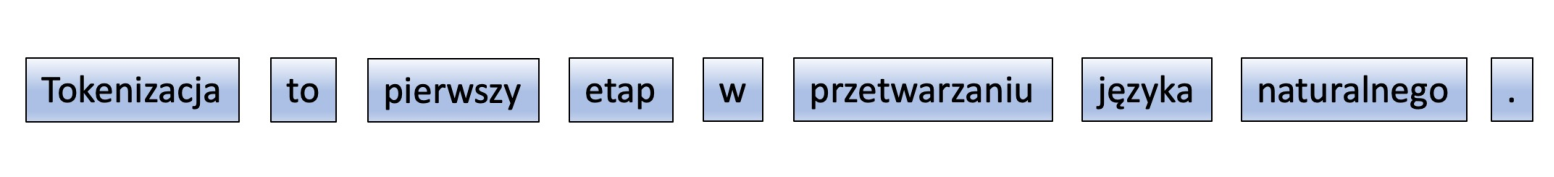
\includegraphics[width=0.95\linewidth]{images/chapter1/tokenizacja.pdf}
	\caption{Zdanie --- Tokenizacja to pierwszy etap w przetwarzaniu języka naturalnego. --- po wykonaniu tokenizacji.}
	\label{fig:tokenizacja}
\end{figure}

\noindent Wygenerowane zostaje tu dziewięć tokenów: \\
$\qquad \rightarrow$ każdy wyraz jest tokenem, \\
$\qquad \rightarrow$  kropka również jest tokenem.


\subsubsection{Normalizacja}
Normalizacja to wykonanie procesów przekształcenia danych tekstowych, które czasami towarzyszą tokenizacji. Normalizacja, inaczej ujednolicenie, może polegać na sprowadzeniu różnych form słów mających podobne (to samo) znaczenie do wspólnej postaci, np. liczebniki znaczące to samo, ale odmienione przez rodzaje --- \textit{jeden}, \textit{jedna}, \textit{jedno} --- należy sprowadzić do postaci \textit{1}, gdyż mają to samo znaczenie. Pominięcie tej procedury skutkowałoby tym, że wyrazy te traktowane by były jako trzy różne słowa mimo, że semantycznie znaczą to samo. Innym zabiegiem normalizacyjnym stosowanym w celu ułatwienia pracy z tekstem jest zamiana wszystkich znaków na znaki tej samej wielkości \cite{normalizacja} --- na wielkie lub małe litery itp. 

\subsubsection{Usuwanie słów-stopów}
Słowa-stopy są to słowa nic nie wnoszące do znaczenia i zrozumienia procesowanych danych (uznawane są za szum). Słowa te (w danym języku) są bardzo powszechnie używane i pojawiają sie właściwie w każdym tekście uniemożliwiając różnicowanie. Wyeliminowanie zbioru tych słów pozwala skupić się na wartościowych treściach (kluczowych słowach umożliwiających skuteczną analizę) \cite{stopwords}. \\
Do słów-stopów zalicza się rodzajniki, spójniki, przyimki itp. Najczęściej są to słowa o najwyższej częstotliwości występowania w tekście. Usuwanie można robić na podstawie dostępnych baz predefiniowanych dla danego języka lub tworzyć własne listy słów-stopów.
Często tworzy się dedykowane listy słów-stopów w zależności od domeny, w której osadzony jest dany tekst. Np., żeby usprawnić analizę tekstu medycznego można usunąć takie słowa jak dr, pacjent itd., żeby analizować wypowiedzi z Twittera można usunąć hashtagi, czyli słowa zaczynające się na \#, nazwy użytkowników --- zaczynające się znakiem @ itp. W ogólności powinno się usuwać wszystkie słowa i frazy, które mają małą moc dyskryminującą i takie, które prowadzą do nieprawidłowości w otrzymywanych wynikach.

%  https://kavita-ganesan.com/what-are-stop-words/#.YQ0ge1MzaL0

\subsubsection{Inne przekształcenia}
Oprócz usuwania słów-stopów można równeż wykonać przekształcenia dające podobny efekt np.
usuwanie akcentów, znaków specjalnych, aposrtrofów, cyfr, czy czegokolwiek niepotrzebnego lub niewnoszącego do zrozumienia niesionej informacji bazując na odpowiednich wyrażeniach regularnych. Przykładem może być usuwanie tagów \verb|HTML|, np. po pobieraniu surowych danych ze strony internetowej (\textit{webscraping}). Przekształcenia te mogą również dotyczyć modyfikacji posiadanych danych. W języku angielskim popularne jest używanie form skrótowych \textit{y'all, I'd, I'll}. Należy je zamienić na \textit{you all}, \textit{I would} oraz na \textit{I will} itd.


\subsubsection{Tworzenie N-gramów}
Tworzenie N-gramów, np. bigramów, trigramów etc. --- polega na tworzeniu połączeń słów, które mogą występować razem. Najpierw się tokenizuje zdanie do słów, a następnie z powstałych tokenów tworzy się N-gramy.
Często zdarza się, że połączenia słów nabierają nowego, innego znaczenia. \\
Przykład: \\
\textit{Nowy Jork} razem ma inne znaczenie niż oddzielne słowa \textit{Nowy} i \textit{Jork}.

\subsubsection{Stemming}
Stemming
to proces usunięcia ze słowa końcówki fleksyjnej (przedrostka, przyrostka) pozostawiając tylko temat wyrazu (nieodmienny rdzeń). Może być przeprowadzany w celu zmierzenia popularności danego słowa. Różne rodzaje stemmerów --- mniej i bardziej agresywne, np. \verb|PorterStemmer| (łagodny), \verb|LancasterStemmer| (bardziej agresywny).

\noindent Wynikiem stemmingu może być ciąg znaków, który sam w sobie nic nie znaczy, ale jest wspólny dla wszystkich słów znaczących to samo w danym tekście jak też normalnym istniejącym i  funkcjonującym słowem. \\
Np. angielskie słowa: \textit{connection}, \textit{connections}, \textit{connective}, \textit{connected}, \textit{connecting} poddane stemmingowi dadzą ten sam wynik, czyli słowo \textit{connect}.

\subsubsection{Lematyzacja}
Lematyzacja to sprowadzenie słowa do jego podstawowej postaci (bazowej), czyli analiza morfologiczna. Do wykonania tego zadania potrzebny jest słownik lub rozbudowany zestaw reguł.
W przypadku czasownika będzie to bezokolicznik, w przypadku rzeczownika --- mianownik liczby pojedynczej. W odróżnieniu od stemmingu --- forma bazowa powstała po lematyzacji zawsze jest  istniejącym słowem.
Warto tutaj dodać, że lematyzacja jest dużo trudniejsza dla silnie fleksyjnych języków ---  takich, które posiadają dużo końcówek dla różnych osób, liczb, przypadków, jak np. język polski. Jest to dużo łatwiejsze w przypadku języka angielskiego.


\subsubsection{Rozpoznawanie części mowy}
Rozpoznawanie części mowy zwane inaczej tagowaniem gramatycznym --- jest to oznaczanie części mowy (POS --- \textit{Part Of Speech}), czyli rozpoznawanie i etykietowanie czy dane słowo jest rzeczownikiem, czasownikiem, przymiotnikiem, przysłówkiem, liczebnikiem itp. Wykonuje się to albo w oparciu o słownik albo wykorzystując występujące końcówki fleksyjne. Może się zdarzyć, że słowo, w zależności od kontekstu, w którym się znajduje, będzie przynależało do różnego typu części mowy . 
\\

\noindent Poniższy przykład dobrze obrazuje wspomnianą niejednoznaczność: \\
$\rightarrow$ \textit{message me} (jako czasownik)
niesie znaczenie daj mi znać lub powiadom mnie, natomiast \\
$\rightarrow$ \textit{a message}  (jako rzeczownik) oznacza po prostu wiadomość.


\subsubsection{Rozpoznawanie bytów nazwanych}
Kolejna operacja na tekście to rozpoznawanie bytów nazwanych. Jest to nic innego jak identyfikowanie/odnajdywanie nazw własnych, które w odróżnieniu od rzeczowników pospolitych, nie są łatwe do rozpoznania, np. lokalizacje, nazwy budynków, dane personalne, waluty, jednostki itp.


\subsubsection{Parsowanie}
Parsowanie to zbieranie indywidualnych „oczyszczonych” kawałków tekstu i grupowanie ich w większe wyrażenia.
Z grubsza, parsowanie można podzielić na dwa rodzaje: parsowanie płytkie (\textit{shallow-parsing}) oraz parsowanie głębokie (\textit{deep-parsing}).

\paragraph{Parsowanie płytkie}
Parsowanie płytkie, czasami określane terminem kawałkowanie (\textit{chunking}), ma na celu wydobycie istotnej informacji, bez potrzeby wyciągania wszystkich zależności składniowych pomiędzy słowami.
Kawałkowanie bierze na wejściu pojedyncze części mowy i zwraca na wyjściu grupy wyrazów/ wyrażenia (\textit{chunki}).
Istnieje 5 głównych rodzajów wyrażeń (grup/\textit{chunków}):
\begin{itemize}
	\item wyrażenia rzeczownikowe (NP),
	\item wyrażenia czasownikowe (VP),
	\item wyrażenia przymiotnikowe (ADJP),
	\item wyrażenia przysłówkowe (ADVP),
	\item wyrażenia przyimkowe (PP).
\end{itemize}

%%%  ------------> obrazek
\begin{figure}[H]
	\centering
	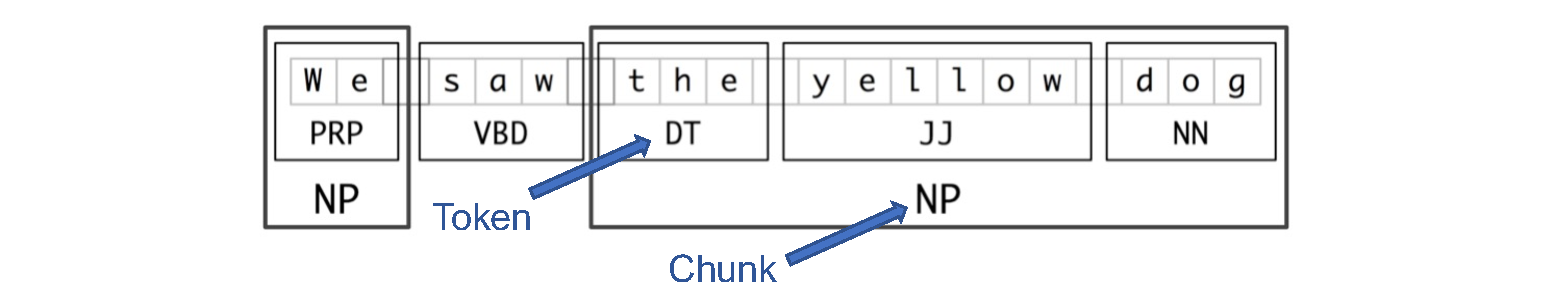
\includegraphics[width=0.95\linewidth]{images/chapter1/shallowParsing.pdf}
	\caption{\href{http://www.nltk.org/book/ch07.html}{Parsowanie płytkie.}}
	\label{fig:shallowParsing}
\end{figure}



\paragraph{Parsowanie głębokie}
Parsowanie głębokie polega na pełnym odtworzeniu drzewa składniowego zdania. 
\\

\noindent Wszystkie wyżej opisane zabiegi stosuje się po to żeby jak najbardziej uprościć budowany model (zmniejszyc jego rozmiary). Jednakże żaden algorytm nie może używać bezpośrednio słów żeby wykoywać modelowanie. Aby budować modele matematyczne, należy przekształcić  słowa w wartości liczbowe (w NLP  w wektory liczb). Gdy dojdzie się do tego punktu, tak naprawdę zabawa się dopiero zaczyna. Można zrobić takie rzeczy, jak wyznaczanie częstotliwości słów w tekście, mierzenie odległości między słowami, wyznaczanie wielu innych przydatnych zależności i parametrów oraz tworzenie modeli klasyfikujących, klasterujących i innych. Istnieje też wiele bibliotek, przy pomocy których można również tworzyć bardzo efektowne wizualizacje.

\section{Podstawy modelowania}
% nazwy bibliotek
%  \verb_sklearn.ensemble.RandomForestClassifier_ 
\subsection{Definicje}
\subsubsection{Uczenie maszynowe}
Uczeniem się systemu jest każda autonomiczna zmiana w systemie zachodząca na podstawie doświadczeń, która prowadzi do poprawy jakości jego działania \cite{cichosz2000}.\\
Uczenie maszynowe to dziedzina nauki dająca komputerom możliwość uczenia się bez konieczności ich jawnego programowania \cite{samuel1959}.  Mówiąc bardziej technicznie uczenie maszynowe polega na tym, że program komputerowy uczy się na podstawie doświadczenia (E) w odniesieniu do jakiegoś zadania (T) i pewnej miary wydajności (P), jeżeli jego wydajność wzrasta wraz z nabywaniem doświadczenia \cite{mitchell}.

\begin{figure}[H]
	\centering
	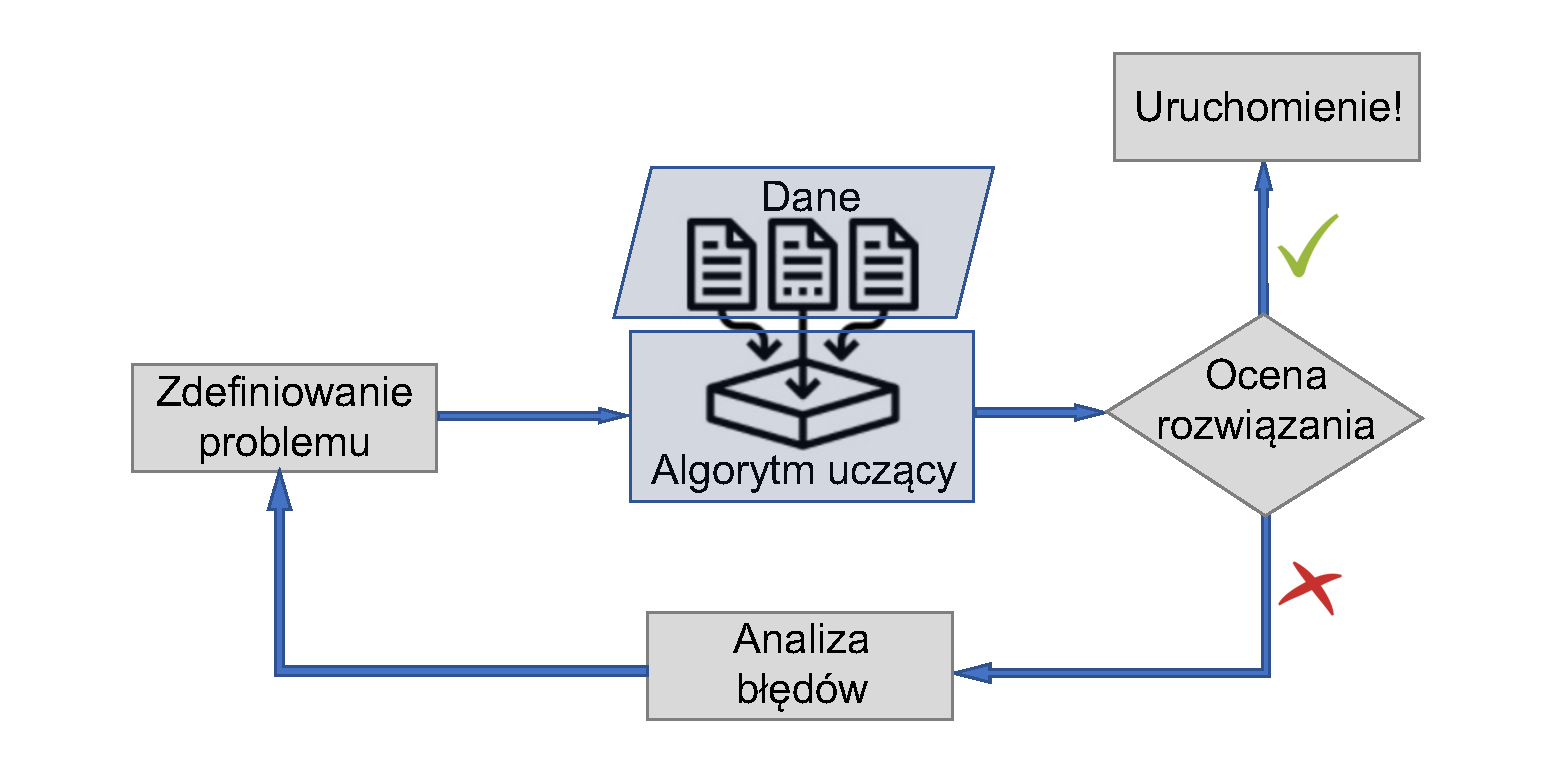
\includegraphics[width=0.75\linewidth]{images/chapter1/machineLearning.pdf }
	\caption{Proces uczenia maszynowego.}
	\label{fig:machine_learning}
\end{figure}


Uczenie maszynowe można podzielić na trzy główne typy:
\begin{enumerate}
	\item Uczenie nadzorowane (\textit{supervised learning}) --- maszyna uczy się generalizować na podstawie oznakowanych danych. W pierwszym etapie nastepuje trenowanie modelu: model jest trenowany na podstawie macierzy cech (\textit{features, atributes}) i odpowiadającym wartościom na wyjściu (\textit{label}). Polega to na dopasowaniu funkcji jak najlepiej odzwierciedlającej dane (generalizującej). Następnie wyznaczony model używa się w predykcji --- na wejściu podaje się macierz z nowymi wartościami cech i wytrenowany model wnioskuje wartość wyjścia (dyskretną --- klasę lub ciągłą --- liczbę) wykorzystując wyuczoną funkcję.
	\item Uczenie nienadzorowane (\textit{unsupervised learning}) --- ma miejsce, gdy informacja trenująca jest niedostępna (brak przynależności do klas wynikowych). De facto używany algorytm sam wyznacza klasy --- znajduje opisy dla tych klas (reguły podziału: jakie klasy są obecne i co je różnicuje) --- i dzieli obserwacje pomiędzy te klasy wg własnego uznania. Proces ten jest często określany mianem grupowania (\textit{clustering}). Należy tu podkreślić, że w zależności od użytego algorytmu, klasy mogą być zdefiniowane w różny sposób --- może istnieć wiele różnych sposobów dzielenia obserwacji na klasy i opisywania każdej klasy, dlatego rodzaj użytego algorytmu ma tu kluczowe znaczenie.
	\item Uczenie wspomagane (\textit{reinforcement learning}).
\end{enumerate}

\subsubsection{Model predykcyjny}
Model predykcyjny opisuje zależności między zmiennymi objaśniającymi (cechami) a zmienną wynikową (targetem) \cite{website}. Umożliwia on, w oparciu o zmienne objaśniające, domniemać jaka jest wartość targetu. Istnieje wiele rodzajów modeli. Przykładami są regresja logistyczna, regresja liniowa, drzewo decyzyjne. \\

\noindent Modele można podzielić ze względu na ich przeznaczenie na:
\begin{itemize}
	\item klasyfikujące --- target dyskretny (np. drzewa decyzyjne, regresja logistyczna),
	\item aproksymujące --- target ciągły (np. regresja liniowa, sieci neuronowe),
	\item asocjujące --- współwystępowanie wartości (np. algorytm A-Priori, sieci asocjacyjne),
	\item segmentujące --- podział na segmenty (np. algorytm k-means, sieci Kohonena).
\end{itemize}

\subsubsection{Klasa}
Klasa --- inaczej target lub zmienna wynikowa lub etykieta --- jest to wartość docelowa wyznaczana przez model predykcyjny, która ma formę dyskretną (nieciągłą).

\subsubsection{Klasyfikacja binarna}
Klasyfikacja binarna --- inaczej regresja logistyczna, to przykład modelu klasyfikacyjnego, w którym na podstawie danych objaśniających nadawane są przynależności do jednej z \textbf{dwóch} możliwych dyskretnych klas wynikowych. Przykładowo na podstawie pewnych określonych charakterystycznych objawów można zakwalifikować pacjenta jako zdrowego lub chorego.

\subsubsection{Algorytm trenujący}
Model może zostać wytrenowany przy pomocy różnych algorytmów trenujących. Algorytmy te mogą różnić się, np. hiperparametrami i ich wartościami oraz dochodzić do wyniku w nieco różny sposób.


\subsubsection{Próbka}
Jest to każdy „element” wykorzystywany do uczenia modelu, tzw. przykład uczący --- pojedyńcza kombinacja cech (atrybutów) wraz z etykietą odpowiadającą tym cechom \cite{geron}. Mówiąc kolokwialnie, jest to jeden wiersz/ rekord/ obserwacja/ obiekt w \verb|Dataframie|.

\subsubsection{Atrybut}
Atrybut --- inaczej cecha (\textit{feature}) --- jest to jeden z aspektów danej próbki. Pojedyńczy atrybut reprezentowany jest jako pojedyńcza kolumna w \verb|Dataframie|. Atrybuty mogą być proste (niepodzielne/ atomowe) lub złożone (można je podzielić na „mniejsze” atrybuty, np. adres zawierający miasto, ulicę, numer, kod pocztowy można rozbić na składowe), kategoryczne lub numeryczne. Atrybuty można również podzielić na niezależne (cechy wykorzystywane do wykonania predykcji) oraz zależne (wyniki predykcji --- tzw. etykiety) \cite{website}.

\subsubsection{Zbiór treningowy}
Zbiór treningowy (\textit{training set}) --- jest to zbiór danych, który używany jest do uczenia się modelu (algorytmu). Na podstawie tych danych model uczy się odpowiednio klasyfikować lub aproksymować wartości wyjścia oraz buduje wszelkie zależności. Inaczej mówiąc, model uczy się przewidywać możliwe wyniki i podejmować decyzje na podstawie przekazanych mu danych \cite{geron}.
\subsubsection{Zbiór testowy}
Zbiór testowy (\textit{testing set}) --- jest to zbiór danych, którego używa się do przetestowania wcześniej wytrenowanego na danych treningowych modelu. Należy podkreslić, że dane zawarte w zbiorze testowym nie mogą być używane wcześniej do nauki modelu (dane, których model nigdy wcześniej nie widział), ponieważ nie będą się wtedy nadawać do obiektywnej oceny działania/skuteczności modelu. Zbioru tego można również użyć w procesie dobierania odpowiedniego zetawu hiperparametrów dla danego modelu \cite{raschka}. \\

\noindent Aby podzielić wyjściowy zbiór danych na treningowy i testowy można użyć popularnej metody \verb|train_test_split| z pakietu \verb|sklearn.model_selection|.


\subsubsection{Hiperparametry}
Zazwyczaj modele w uczeniu maszynowym posiadają parametry. Niektóre mają ich więcej drugie mniej --- w zależności od złożoności danego modelu. Gdy wartość parametru obliczana jest samodzielnie przez algorytm podczas procesu trenowania to parametr taki nazywamy po prostu zwykłym parametrem, natomiast jeżeli wartość parametru zostaje podana przez modelarza, który danego algorytmu używa, to taki specjalny parametr nosi miano hiperparametru \cite{mamczur}. Przykładem hiperparametrów (zewnętrznych parametrów) są, np. głębokość lasu losowego (liczba drzew) czy liczba epok treningowych, natomiast zwykłymi (wewnętrznymi) parametrami mogą być wagi w sieciach neuronowych, czy współczynniki w regresji liniowej.


\subsubsection{Funkcja kosztu (straty)}
Tworzony model, czyli de facto funkcja dopasowywana do danych wejściowych modelu zwana jest powszechnie hipotezą. Dokładność funkcji hipotezy (w stosunku do zbioru uczącego) można zmierzyć za pomocą funkcji kosztu. Przykładem funkcji kosztu może być średni kwadratowy błąd (\textit{mean squared error}). W dużym skrócie, funkcja kosztu zwraca średnią różnicę między wynikami funkcji hipotezy a rzeczywistymi danymi wyjściowymi dla każdego wejścia.
Celem jest minimalizacja tej funkcji kosztu, czyli znalezienie odpowiednich optymalnych parametrów. Im mniejsza wartość funkcji kosztu, tym dokładniejsza jest funkcja hipotezy, czyli lepiej dopasowany jest nasz model \cite{andrewng}.

%\textcolor{TODO}{Dopisać może wzór przykładowej funkcji kosztu z Andrew Ng}

% https://ichi.pro/pl/uczenie-maszynowe-funkcje-kosztow-88976465788030


\subsubsection{Błąd}
Błąd jest to różnica pomiędzy wartością otrzymaną a wartością rzeczywistą (prawdziwą) dla danej obserwacji. Technicznie, błąd można wyznaczać na wiele różnych sposobów. Najczęściej błąd podaje się jako uśrednioną wartość błędów obliczoną dla całego zbioru danych.

\subsubsection{Walidacja --- metryki sukcesu (\textit{model evaluation metrics})}
 Walidacja jest to proces oceny przydatności danego modelu. Do walidacji działania stworzonego modelu stosuje się różne metryki sukcesu. Sa to takie wielkości, które mówią jak dobrze dany model nauczył się generalizować, a co za tym idzie pozwalają nam określić przydatność danego modelu do wykonywania określonego zadania. W problemach klasyfikacyjnych często do oceny używa się macierzy omyłek, która posiada informacje o prawidłowo i nieprawidłowo sklasyfikowanych przykładach w odniesieniu do prawdziwych wartości dla danych przykładów. W oparciu o nią można później obliczyć różne metryki sukcesu. Bardzo popularną metryką jest precyzja (\textit{accuracy}) --- obliczana jako liczba dobrze sklasyfikowanych przykładów do liczby wszystkich przykładów.

\subsubsection{Przeuczenie (\textit{overfitting})}
Przeuczenie (\textit{overfitting}) polega na tym, że model przesadnie dopasowuje się do konkretnych danych --- tych, na podstawie których został zbudowany. Dla tych konkretnych danych zwraca on wyniki obdarzone bardzo małym błędem, natomiast nie umie on dobrze generalizować, a co za tym idzie, jeżeli nakarmimy model nowymi danymi otrzymamy znacznie gorsze wyniki. Przeuczenie następuje, gdy model statystyczny ma zbyt dużo parametrów w stosunku do rozmiaru próby, na podstawie której był konstruowany \cite{overfitting}.

%%%  ------------> obrazek
\begin{figure}[H]
	\centering
	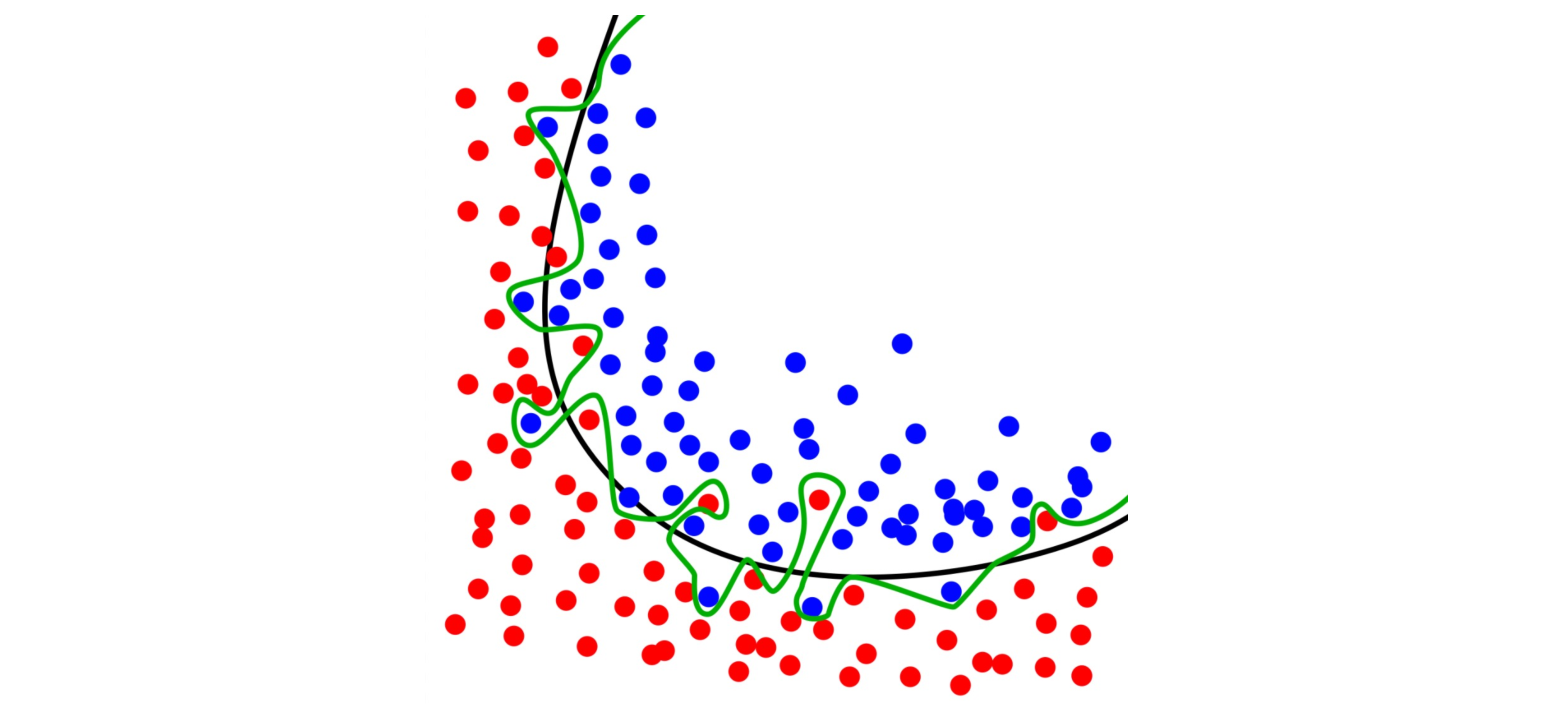
\includegraphics[width=0.95\linewidth]{images/chapter1/overfitting.pdf}
	\caption{\href{https://upload.wikimedia.org/wikipedia/commons/1/19/Overfitting.svg}{Przeuczenie (overfitting).}}
	\label{fig:overfitting}
\end{figure}

\noindent Zielona linia reprezentuje model przesadnie dopasowany (przeuczony), a czarna linia reprezentuje model uregulowany. Chociaż zielona linia najlepiej podąża za danymi treningowymi, jest zbyt zależna od tych danych i prawdopodobnie będzie miała wyższy poziom błędów w przypadku nowych danych w porównaniu z czarną linią. Czarna linia zdecydowanie lepiej generalizuje.



\subsubsection{Wektoryzacja tekstu}
Większość istniejących algorytmów trenujących modele predykcyjne wymaga na wejściu wektorów liczbowych. Istnieje wiele technik pozwalających zamienić tekst na wektor liczb rzeczywistych. Najprostszą techniką jest użycie wektoryzacji zliczeniowej (\textit{Count Vectorization).} Wg dokumentacji \verb|ScikitLearn|, wektoryzacja ta polega na konwersji kolekcji dokumentów tekstowych na macierz zawierającą zliczenia poszczególnych tokenów \cite{countVectorizer}. Mówiąc prościej, polega na zliczaniu słów w danym tekście (korpusie) i w rezultacie umożliwia obliczenie częstości występowania danego słowa w analizowanym tekście. Zaimplementowana jest ona w pakiecie \verb|sklearn.feature_extract-| \verb|ion.text.CountVectorizer|. Rozkład częstości słów można wizualizować przy pomocy wykresów używając metody \verb|FreqDistVisualizer| z pakietu \verb|yellowbrick.text|.\\
